\section{Deskriptiv}
Das Experiment welches in \ref{Sec:Experiment} beschrieben wurde, wurde mit verschiedenen AV Scannern wiederholt. Sinnvolle Ergebnisse haben dabei nur die Microsoft Scanner ergeben, unter denen der klassische Windows Defender und der für die Anwendung des Tools wichtige Microsoft Defender in der Enterprise Edition waren. Weitere Scanner mit denen das Experiment gestartet wurden, waren Deep Instinct, Cylance und Trellix. Diese konnten aber die PE Files nicht ausführen und somit keinen Scan durchführen. Ob dies an den Scannern, ungünstigen Ergebnissen des GAs oder an Fehlern in der Pipeline (\ref{Sec:Technologie}) liegt, wurde nicht weiter untersucht, da eine Aussage für den Use Case und die Studie bereits möglich waren.
Im den folgenden Diagrammen sind die Ergebnisse aus jeweils drei Durchläufen pro Scanner notiert, nach denen der Cache für den GA geleert wurde. Die Experimente wurden in einem Fall (Shell bei MDE Scanner) wiederholt, da es zu keinem Ergebnis kam. In der Datengrundlage wurden dann die Laufzeiten beider Ausführungen addiert und der Cache dazwischen nicht geleert. In allen anderen Fällen hat eine Durchführung gereicht, um mindestens eine Evasion-Sample zu erhalten.


\begin{figure}[h]
    \centering
    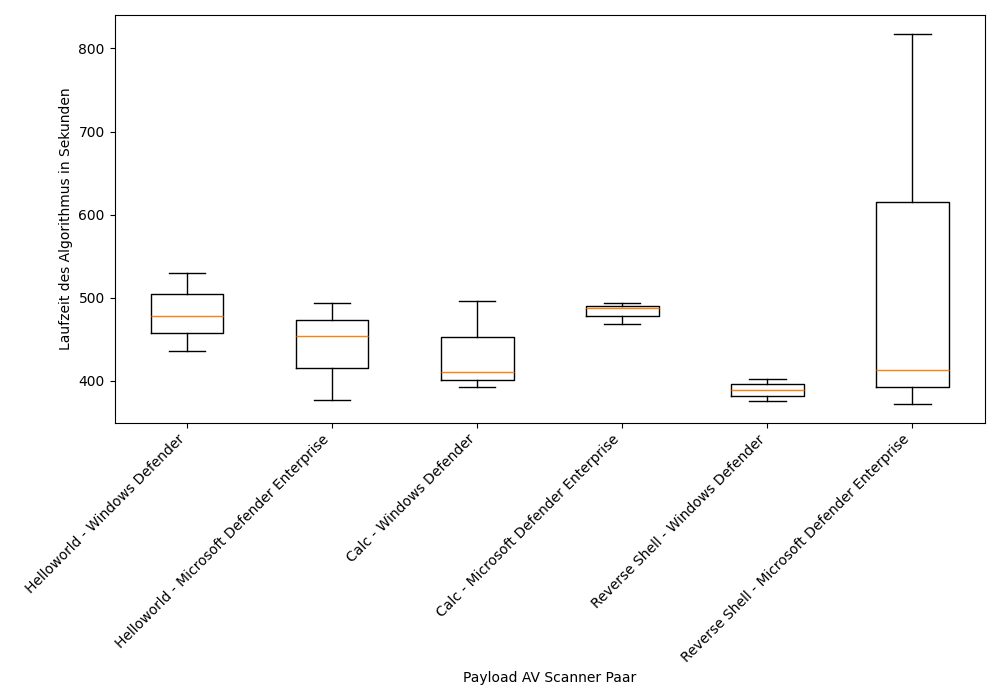
\includegraphics[width=0.85\textwidth]{gfx/Desktriptiv/time_overview.png}
    \caption{Laufzeit der Experimente}
    \label{fig:runtime_overview}
\end{figure}

\begin{figure}[h]
    \centering
    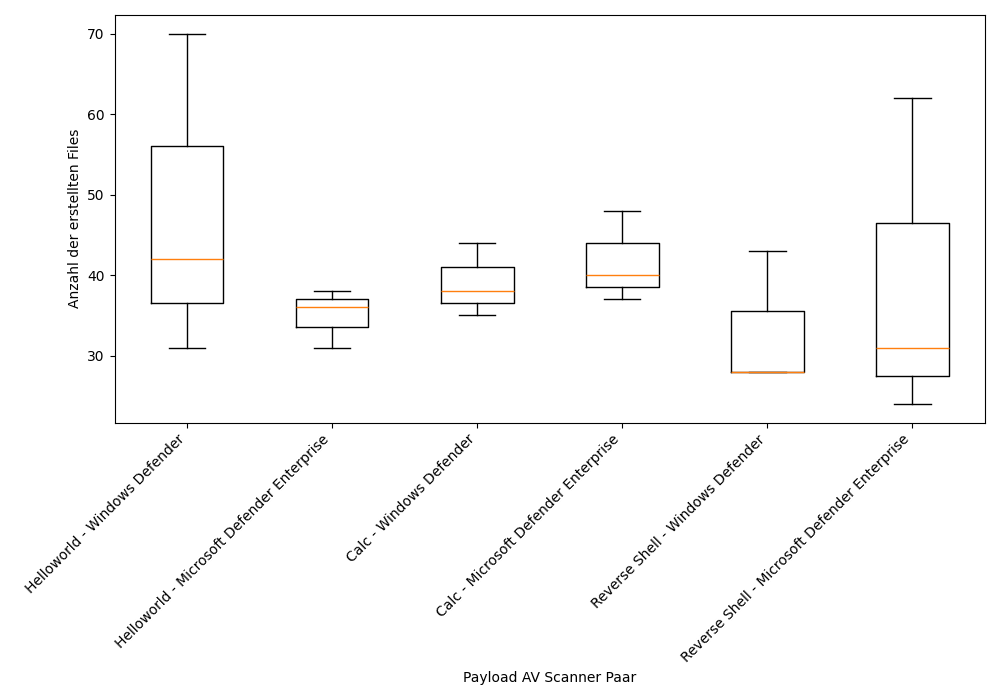
\includegraphics[width=0.85\textwidth]{gfx/Desktriptiv/files_overview.png}
    \caption{Erstellte Files pro Experimente}
    \label{fig:files_overview}
\end{figure}
\begin{figure}[h]
    \centering
    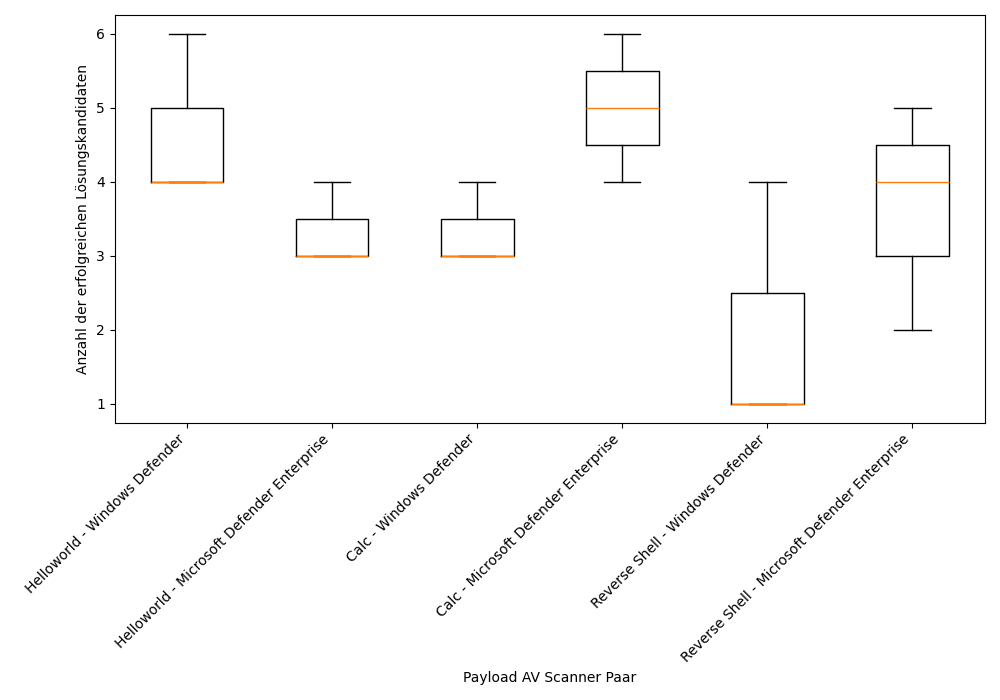
\includegraphics[width=0.85\textwidth]{gfx/Desktriptiv/evaded_overview.png}
    \caption{Anzahl erfolgreicher Obfuskierungen}
    \label{fig:evaded_overview}
\end{figure}
\begin{figure}[]
    \centering
    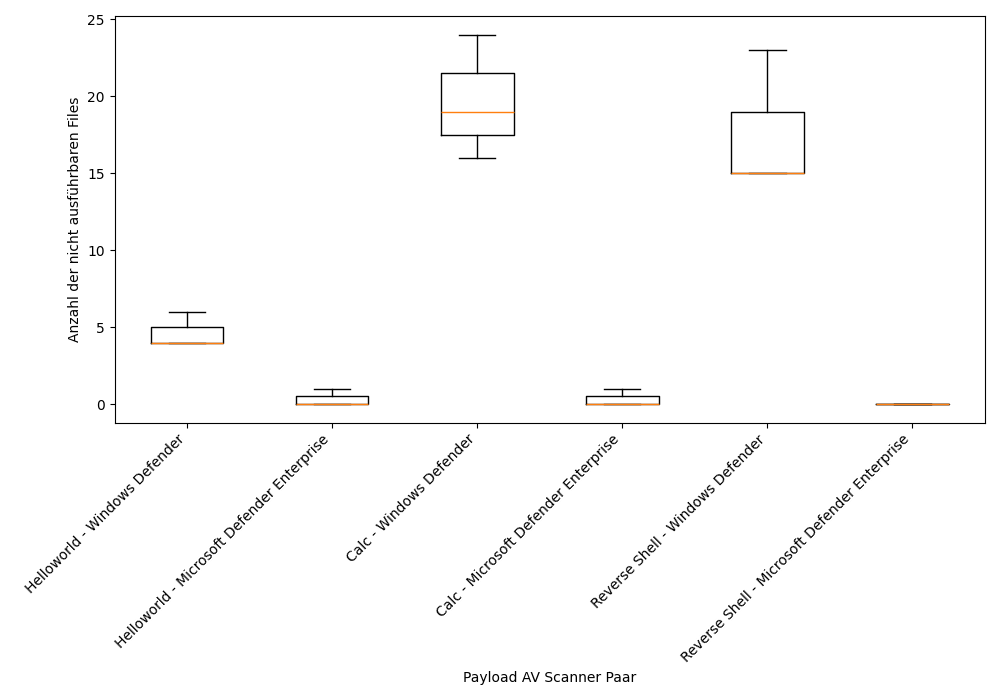
\includegraphics[width=0.85\textwidth]{gfx/Desktriptiv/corrupt_overview.png}
    \caption{Anzahl der Korrupten Dateien}
    \label{fig:corrupt_overview}
\end{figure}
\begin{figure}[h]
    \centering
    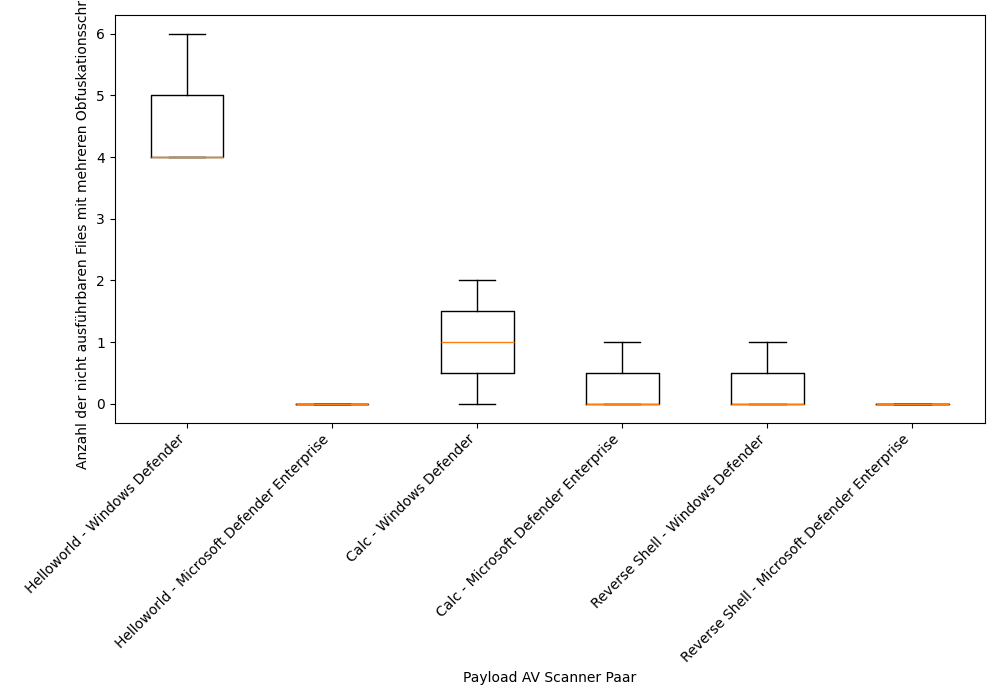
\includegraphics[width=0.85\textwidth]{gfx/Desktriptiv/multicor_overview.png}
    \caption{Anzahl der korrupten, mehrstufigen Obfuskierungen}
    \label{fig:multicor_overview}
\end{figure}

Eine wohlwollende Schätzung anhand dem Verhältnis von erfolgreichen Lösungskandidaten und der Laufzeit des Algorithmus gibt uns eine Abschätzung der Laufzeit pro erfolgreicher Lösung des Obfuskationsproblems, wie man sie in Abbildung \ref{fig:time_per_evasion} sehen kann. Diese Werte ermöglichen eine Einschätzung der Performance des Algorithmus in seiner produktiven Umgebung, wenn eine einzige Lösung ausreichend ist, eröffnet aber auch die Möglichkeit, weitere Lösungen für das vorhandene Problem zu finden.
\begin{figure}[h]
    \centering
    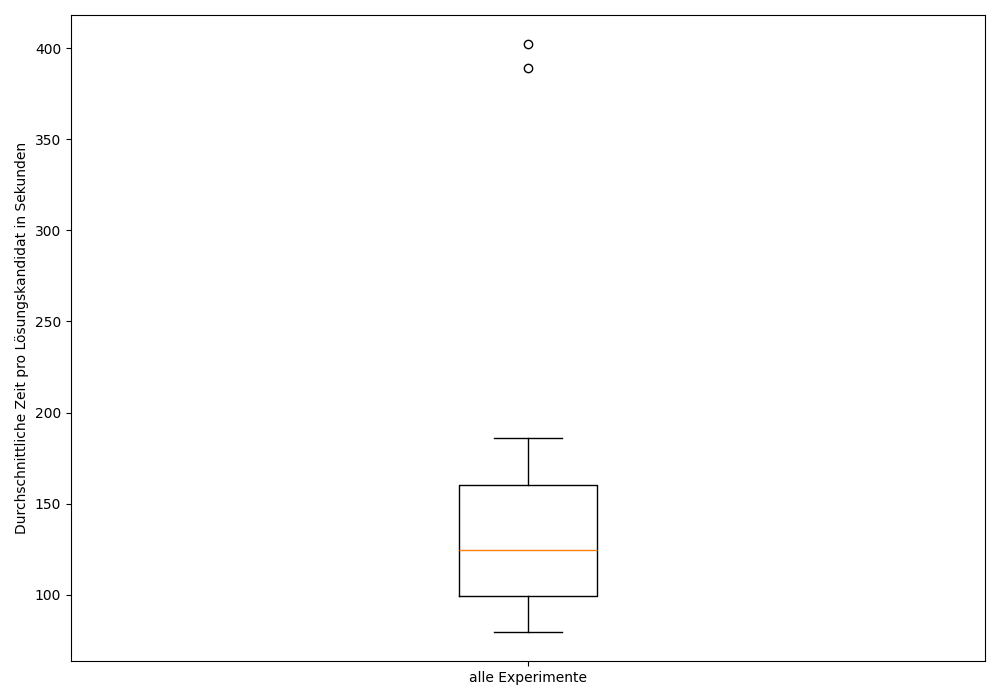
\includegraphics[width=0.85\textwidth]{gfx/Hypothesendiagramme/time_per_evasion.png}
    \caption{Zeit pro Lösung}
    \label{fig:time_per_evasion}
\end{figure}